\RequirePackage[l2tabu, orthodox]{nag}

\documentclass{article}

\usepackage[utf8]{inputenc}
\usepackage[ngerman]{babel}

\usepackage{natbib}
\usepackage{graphicx}
\usepackage{capt-of}
\usepackage[colorlinks,pdfpagelabels,pdfstartview=FitH,bookmarksopen=true,bookmarksnumbered=true,linkcolor=black,plainpages=false,hypertexnames=false,citecolor=black]{hyperref}
\usepackage{caption}
\usepackage{subfigure}
\usepackage{listings}
\usepackage{microtype}

% http://tex.stackexchange.com/questions/167948/package-rerunfilecheck-warning-file-out-has-changed
\usepackage{bookmark}

% gantt charts: http://ctan.mirrorcatalogs.com/graphics/pgf/contrib/pgfgantt/pgfgantt.pdf
\usepackage{pgfgantt}

% change margins to 2.5 cm and enable landscape
\usepackage[margin=3cm]{geometry}
\usepackage{pdflscape}

\usepackage{tabulary}

% place figures at exactly the position given in the code
\usepackage{float}

% custom counters for lists
\usepackage{enumitem}

% table columns with background shading
\usepackage{colortbl}

\newcommand{\appname}{Flashcard-Website}


\begin{document}
\begin{titlepage}
    \large
    \begin{flushleft}
        Web Engineering, 2. Semester \\
        Projektmanagment, 2. Semester \\
        TINF13B2
    \end{flushleft}
    
    \vfill

    \begin{center}
    	% H. Balzert, Lehrbuch der Software-Technik
        \Huge SOLL-/IST-Analyse\\
        \Large \appname \\
        \vspace{1cm}
        \normalsize David Ehlen (5460297),\\
        Julien Hadley Jack (4739854), \\
        Sebastian Dernbach (9586963), \\
        \vspace\medskipamount
        \vspace\medskipamount
        Karlsruhe, 07.07.2014
    \end{center}
    
    \vfill
    
    \begin{flushright}
        Duale Hochschule \\
        Baden-Württemberg \\
        \vspace\medskipamount
        Betreuer: Jörn Eisenbiegler,\\
        Simone Freudenmann
    \end{flushright}
\end{titlepage}

\newpage

% removes the page numbers for the toc
\pagestyle{empty}
\addtocontents{toc}{\protect\thispagestyle{empty}}
\tableofcontents
\cleardoublepage

% normal page numbering for the rest of the document
\setcounter{page}{1}
\pagestyle{plain}
\setcounter{page}{1}

\section{Projektstrukturplan}
\subsection{Zielbestimmung}
Das Endprodukt setzt alle Musskriterien um. Außerdem wurden noch drei Wunschkriterien erfüllt:
\begin{description}
	\item[/WK10/] Für jedes Karteikartenset werden Statistiken angezeigt (Erfolgsquote,...).
	\item[/WK20/] Mathematische Ausdrücke werden in natürlicher Form (z.b. \( e^{\frac{3}{4}\pi i}\)) dargestellt.
	\item[/WK30/]\label{bilder} Bilder können eingefügt werden.
\end{description}

\noindent Hierbei kann man bei \textbf{/WK30/} nur Bilder über die URL einbetten, aber nicht neue Bilder zu dem Server hochladen.

\subsection{Nichtfunktionale Anforderungen}
Die nichtfunktionalen Anforderungen wurden soweit wie möglich getestet.

\subsection{Qualitätsanforderungen}


\begin{center}
\begin{tabular}{|>{\columncolor[gray]{0.8}}l|r|r|}
\hline 
\textbf{Produktqualität} & \textbf{SOLL} & \textbf{IST} \\ 
\hline 
Richtigkeit & sehr gut & gut \\ 
\hline 
Verständlichkeit & sehr gut & sehr gut \\ 
\hline 
Bedienbarkeit & sehr gut & sehr gut\\ 
\hline 
Zeitverhalten & sehr gut & sehr gut\\ 
\hline 
Stabilität & gut & sehr gut \\ 
\hline 
Anpassbarkeit & gut & gut \\ 
\hline 
Installierbarkeit & sehr gut & sehr gut \\ 
\hline 
Fehlertoleranz & gut & gut \\ 
\hline 
Austauschbarkeit & sehr gut & sehr gut \\ 
\hline 
\end{tabular}
\end{center}

\noindent Die Richtigkeit konnte leider nicht erreicht werden. Dies lag hauptsächlich, dass wir uns in der Planung für den WYSYWYG-Editor TinyMCE entschieden hatten. Dieser hat uns aber viele Probleme bereitet.

Es kam öfters vor, dass wir ihn in mehreren Testfälle mit korrekten Endergebnissen testen konnten. Aber als wir sie zu einem späteren Zeitpunkt wiederholten, traten plötzlich Probleme auf, obwohl am Code und am Server nichts verändert worden ist. Viele Fehler konnten im Code beseitigt werden, aber leider nicht alle. In diesen Fällen wird es meist durch ein Neuladen der eigenen Seite kurzzeitig behoben.

\subsection{Testfälle}
Die Testfälle der Musskriterien und erfüllten Wunschkriterien wurden mit verschiedenen Browser getestet. Dies hat uns geholfen einige Fehler noch zu finden. Unterschiede zwischen z.B. Google Chrome und Mozilla Firefox führten zu unterschiedlichen Darstellungen. Wenn möglich wurde dies behoben.

\section{Terminplan}
Wir haben uns für Amazon AWS entschieden zur Bereitstellung des Servers. Dies ermöglicht eine einfache Kollaboration zwischen den Mitarbeitern und lässt die Webseite mit der Anzahl der Besucher skalieren. Dieser Dienst wird auch von Firmen wie NASA, Pinterest und Netflix für ihre produktiven Dienste benutzt.
Dabei hatten wir mit komplexeren Themen wie Firewallregeln und Benutzerverwaltung öfters Probleme. Diese waren nicht eingeplant, so dass das Projektende um 2 Tage überschritten wurde. Da aber ein Puffer zwischen Projektende und Abgabetermin der Dokumentation mitkalkuliert war, konnte dieser Termin ohne Schwierigkeiten eingehalten werden.


\section{Ressourcenplan}
Die Zusammenarbeit zwischen den Mitgliedern des Projektes hat gut funktioniert. Ein Vorteil war, dass sich die Studenten während der Projektphase in ihrer Theoriephase befanden. Das bedeutet, dass sie sich täglich gesehen haben und dadurch oft über ihren Stand und ihre Problemen ausgetauscht haben.

\smallskip
\noindent Es gab keine Ausfälle von Arbeitskräften durch Krankheiten oder aus anderen Gründen.

\smallskip
\noindent Das Projekt konnte mit den geplanten Ressourcen umgesetzt werden.

\section{Kostenplan}

Während des Projektes erhielt der Miterarbeiter, der für die Serveradministration zuständig war, eine E-Mail von Amazon. Es enthielt eine Warnung wegen verdächtigen Aktivitäten auf dem Amazon-AWS-Account. Der Mitarbeiter hat danach beim Überprüfen Änderungen von einer unerlaubten Drittperson auf dem Account entdeckt.

Nach einer mehrstündigen Fehlersuche konnte der Weg festgestellt werden, wie diese Person Zugang erlangen konnte: 

Der Code des Projektes war in einem öffentlichen Versionskontrollsystem auf www.github.com veröffentlicht. Die Datei mit den nötigen Login-Daten für das Amazon-AWS-Account wurde einem Filter hinzugefügt, damit sie nicht veröffentlicht wird. Ein Mitarbeiter hatte Software verwendet, um seine Änderungen dem Versionskontrollsystem hinzuzufügen, die diesen Filter nicht benutzte.

Da Amazon AWS für kleine bis riesigen Webseiten verwendet werden kann, gibt es auch kostenpflichtige Optionen. Die unerlaubte Person hat eine Vielzahl von den Optionen dazugebucht. Obwohl er nur Zugriff für einen Tag hatte, konnte er eine Rechnung von 568,14 USD in dieser Zeit für den Mitarbeiter ansammeln.

\begin{figure}[H]
    \centering
    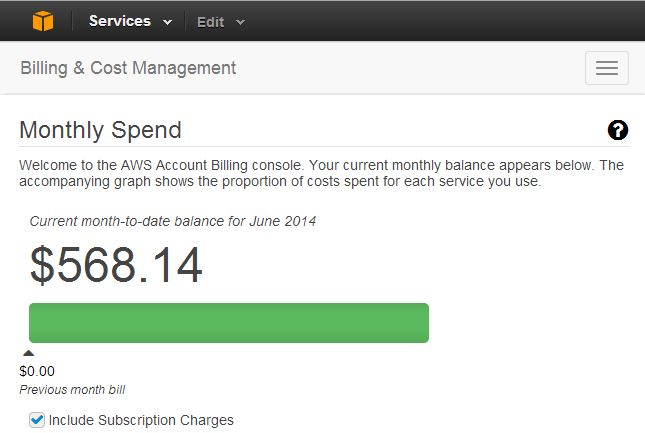
\includegraphics[width=0.7\textwidth]{images/amazon-bill.jpg}
    \caption{Rechnung Amazon AWS}
    \label{fig:bill}
\end{figure}

\noindent Nach einem Gespräch mit dem Kundenservice von Amazon waren sie freundlicherweise bereit die Kosten zu erstatten. Dadurch waren die Gesamtkosten am Ende wie geplant.

Um es in zukünftigen Projekten zu vermeiden, könnte man die Zugriffsrechte für die Mitarbeiter weiter eingeschränkt. Außerdem sollte man in Zukunft einen Server-Anbieter auswählen, bei dem man eine obere Kostenschranke einrichten kann.

\section{Risikoplan}

Durch eine integrierte Fehlerverarbeitung haben wir verhindert, dass der Nutzer durch nicht abgefangene Fehler verwirrt wird. Es kam ebenfalls zu keinem krankheitsbedingten Verlust während des gesamten Projektzeitraums. Auch das Risiko eines Serverausfalls haben wir durch den Einsatz des Amazon AWS Services gemindert.

\section{Kommunikationsplan}

\begin{figure}[H]
    \centering
    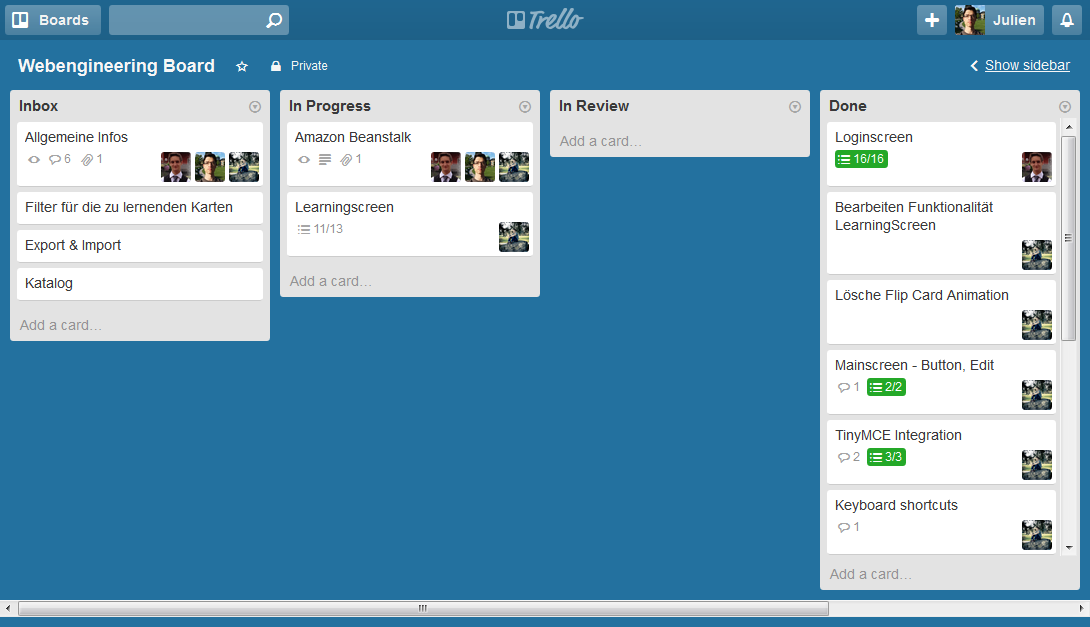
\includegraphics[width=0.8\textwidth]{images/trello.png}
    \caption{Trello}
    \label{fig:trello}
\end{figure}

Der Kommunikationsplan wurde durch alle Projektbeteiligten eingehalten. Darüber hinaus war eine ständige Kommunikation durch die täglichen Besuche der Dualen Hochschule, öfters stattfindende Online Video Meetings via Google Hangout und durch unser Projektmanagement Tool Trello gegeben. Durch das von Trello zur Verfügung gestellte Kanban Board konnte jeder selbst den aktuellen Aufgabenstatus der anderen Mitarbeiter nachlesen. 

\section{Persönliche Einschätzung}

\begin{figure}[H]
    \centering
    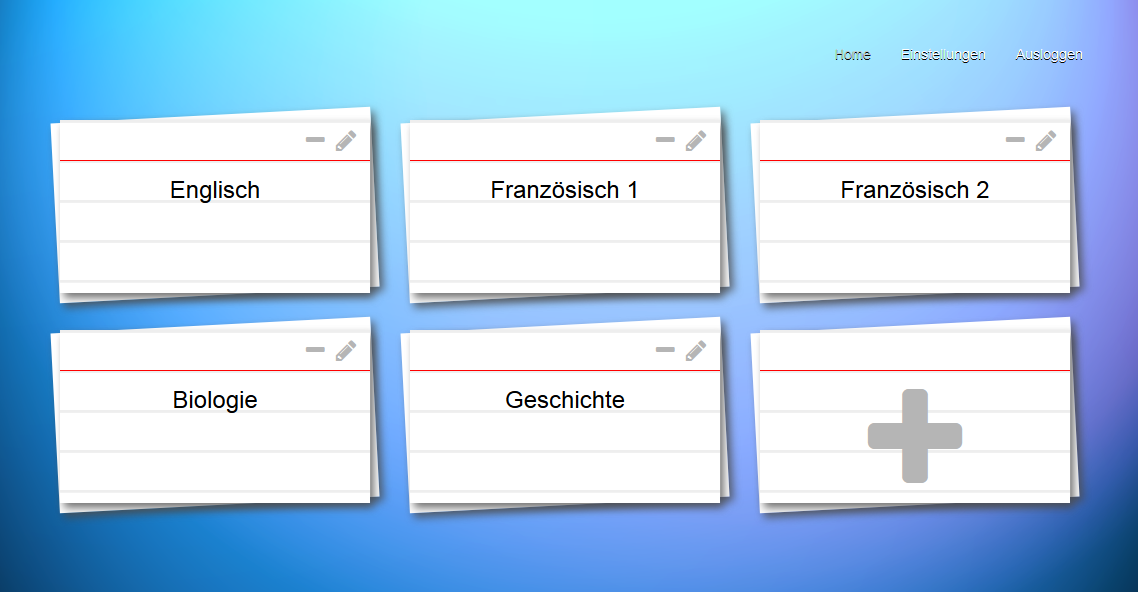
\includegraphics[width=0.8\textwidth]{images/overview.png}
    \caption{Hauptbildschirm}
    \label{fig:dashboard}
\end{figure}

Das obige Bild zeigt den aktuellen Hauptbildschirm der Karteiverwaltung. Die Oberfläche wurde wie geplant umgesetzt und versucht mit Skeuphorismen zu designen, sodass für den Benutzer die Parallele zum Lernen mit ``Stift und Papier`` gegeben ist. Dadurch erhoffen wir uns auch Benutzer anzusprechen, die dem Lernen am Computer skeptisch gegenüber stehen.

Besonders durch jene Designwahl wurde unsere Entscheidung für das Karteikartenprojekt bestätigt, da dieses Raum für kreatives Arbeiten ermöglichte, was rückblickend dazu führte, dass mit besonderer Freude und dem daraus resultierenden Engagement gearbeitet werden konnte.

\begin{figure}[H]
    \centering
    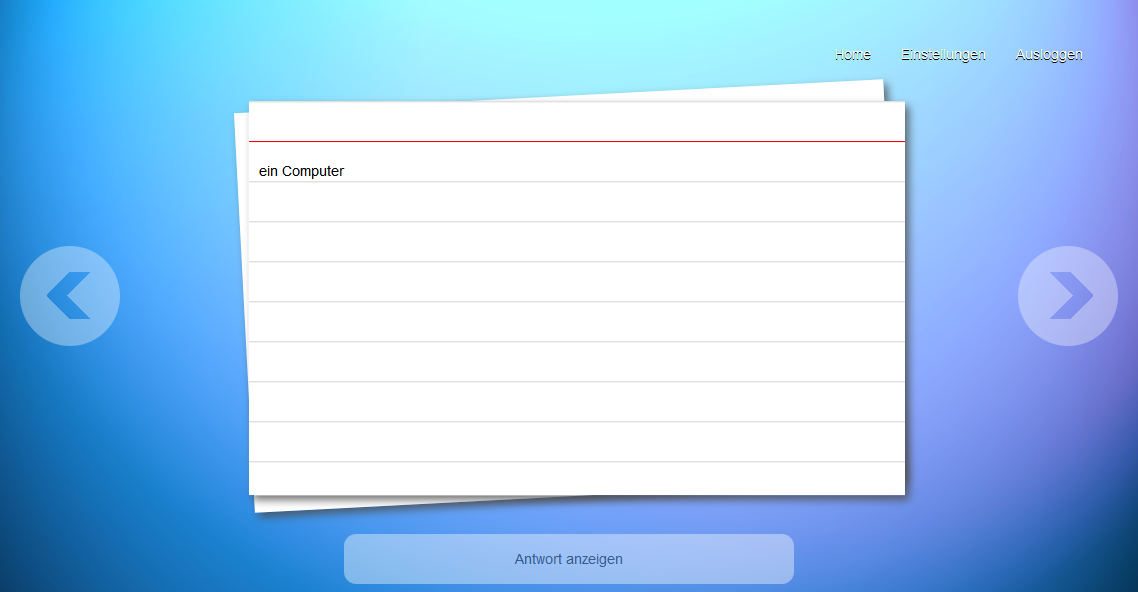
\includegraphics[width=0.8\textwidth]{images/learningscreen-answer.png}
    \caption{Frageseite einer Karteikarte}
    \label{fig:learning-question}
\end{figure}

Das zweite hier angeführte Bild zeigt den ``Lernbildschirm``. Hier kann ein bestehendes Karteikartenset gelernt und angeschaut werden. Die Implementierung war rückblickend etwas schwieriger als erwartet, da mehrere Funktionalitäten wie das Editieren, Hinzufügen und Löschen von Karteikarten gegeben sein muss, damit das Projekt zumindest die minimale Anforderungen an ein Online-Lernsystem erfüllt, jene Funktionalitäten die auch in unseren Musskriterien verankert sind. Durch Unterschiede in den gängigen Browsern mussten hier viele individuelle Konfigurationen getätigt werden.

Besonders beschäftigte uns das gleichzeitige Arbeiten an einem Projekt durch mehrere Teammitglieder. Sowohl das Aufsetzen eines Versionierungssystems, als auch das Aufsetzen einer Infrastruktur (durch den Amazon Beanstalk Server) waren mit viel Arbeit verbunden. Durch die aufgesetzte Umgebung war es uns so möglich, mit den gleichen Bedingungen simultan an dem Projekt arbeiten zu können, und eventuell auftretende Fehler bei einem der Teammitglieder, oder deren Aktivitäten bezüglich des Projektes, nachzuvollziehen.

\newpage
\section{Ehrenamtliche Erklärung}

Ich erkläre ehrenwörtlich,
\begin{itemize}
    \item dass ich meine Projektarbeit selbständig geplant und durchgeführt habe;
    \item dass ich die Übernahme wörtlicher Zitate aus der Literatur sowie die Verwendung der Gedanken anderer Autoren an den entsprechenden Stellen innerhalb der Arbeit gekennzeichnet habe;
    \item dass ich meine Projektarbeit bei keiner anderen Prüfung
    vorgelegt habe.
\end{itemize}
Ich bin mir bewusst, dass eine falsche Erklärung rechtliche Folgen haben wird. \\

\vspace{1cm}
Karlsruhe, 05.07.2014 

\end{document}